\documentclass[aspectratio=169]{beamer}
\geometry{paperwidth=160mm,paperheight=100mm}
\usepackage{beamerthemesidebar}
\usepackage{hyperref}
\usepackage{color}
\usepackage{multimedia}
\usepackage{colortbl}
\usepackage{amsmath}
\usepackage{empheq}
\usepackage{cancel}
\usepackage{amssymb}
\usepackage{amsfonts}
\usepackage{lipsum}
\usepackage{tcolorbox}
\usepackage{tabularx}
\usepackage{caption}
\usepackage{bm}

\setbeamersize{sidebar width right=0pt}
\setbeamertemplate{footline}[frame number]
%
\definecolor{orange}{RGB}{250,167,12}
\definecolor{yellow}{RGB}{246,250,12}
\definecolor{green}{RGB}{128,238,1}
\definecolor{black}{RGB}{0,0,0}
\definecolor{blue}{RGB}{0,0,255}
\definecolor{red}{RGB}{255,0,0}
\definecolor{sepia}{RGB}{94,38,18}
\newcommand{\ve}[1]{{\rm\bf {#1}}}
\newcommand{\q}[1]{\textcolor{blue}{#1}}
\newcommand{\blue}[1]{\textcolor{blue}{#1}}
\newcommand{\sepia}[1]{\textcolor{sepia}{#1}}
\newcommand{\red}[1]{\textcolor{red}{#1}}
\newcommand{\green}[1]{\textcolor{green}{#1}}
\newcommand{\yellow}[1]{\textcolor{yellow}{#1}}
\newcommand{\orange}[1]{\textcolor{orange}{#1}}
\definecolor{burlywood}{RGB}{255,211,155}
\definecolor{chocolate}{RGB}{255,127,36}
\definecolor{tan}{RGB}{210,180,140}
%
\def\onethird{{\textstyle{1\over3}}}
\def\twothirds{{\textstyle{2\over3}}}
\def\fourthirds{{\textstyle{4\over3}}}
\def\onehalf{{\textstyle{1\over2}}}
\def\threehalfs{{\textstyle{3\over2}}}
%
\newcommand{\pd}{\partial}
\newcommand{\aMLT}{\alpha_{\rm MLT}}
\newcommand{\Fconv}{F_{\rm conv}}
\newcommand{\Frad}{F_{\rm rad}}
\newcommand{\Ftot}{F_{\rm tot}}
\newcommand{\Hp}{H_p}
\newcommand{\prad}{p_{\rm rad}}
\newcommand{\pgas}{p_{\rm gas}}
%
\title{Theoretical Astrophysics I: Physics of Sun and Stars\\
Lecture 6: Radiative Energy Transport}
\author{\texorpdfstring{\sepia{Petri K\"{a}pyl\"{a} Ivan Mili\'{c}}\newline\blue{\url{pkapyla, milic@leibniz-kis.de}}}{}}
\institute{Institut f\"ur Sonnenphysik - KIS, Freiburg}
\date{\today}
%
\begin{document}
\frame{\titlepage}

% Few general remarks on photons vs particles 
% Description of radiation field: angle and wavelength dependence
% RTE Kirchoffs Law, Planck Law
% optical depth, source function etc. 
% Few simple solutions 
% Diffusion approximation
% Opacity sources 
% Misc 


\section{General remarks}
%
\frame{
\frametitle{Brief recap}
\begin{minipage}{0.55\linewidth}
\begin{itemize}
\item We started with describing observed properties of the stars. One quantity that we measure (and want to reproduce) is the \textbf{luminosity}, and conversely \textbf{flux} (or specific flux).
\item We wrote down equations that govern stellar structure and evolution. Solving them for proper boundary conditions will yield the structure of a star: $p(r)$, $T(r)$, $\rho(r)$, $F(r)$, etc...
\item Analyzing their variation in time allows us to model stellar evolution.
\item We spent last two lectures talking about a difficult problem of convection. But there is another way to transport energy: via \textbf{radiation}.
\end{itemize}
\end{minipage}
\begin{minipage}{0.44\linewidth}
\begin{figure}
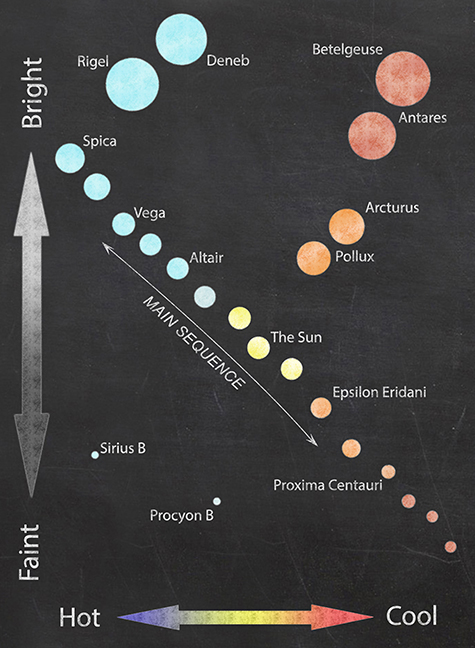
\includegraphics[width=6cm]{figures/hr_simple.jpg}
\caption*{HR diagram}
\end{figure}
\end{minipage}
}
%
\frame{
\frametitle{Photons vs particles}
\begin{minipage}{0.5\linewidth}
\begin{itemize}
\item It is obvious that radiation can carry energy. 
\item We treat radiation using photons, but they are clearly different from atoms, molecules, ions and electrons. 
\item Photons do not have mass and move with speed of light. 
\item The number of photons is not conserved. 
\item Photons can also be treated like a gas (e.g. see the derivation of Stefan-Boltzmann law by Boltzmann)
\item They still observe conservation of energy, momentum, angular momentum, etc.
\end{itemize}
\end{minipage}
\begin{minipage}{0.49\linewidth}
\begin{figure}
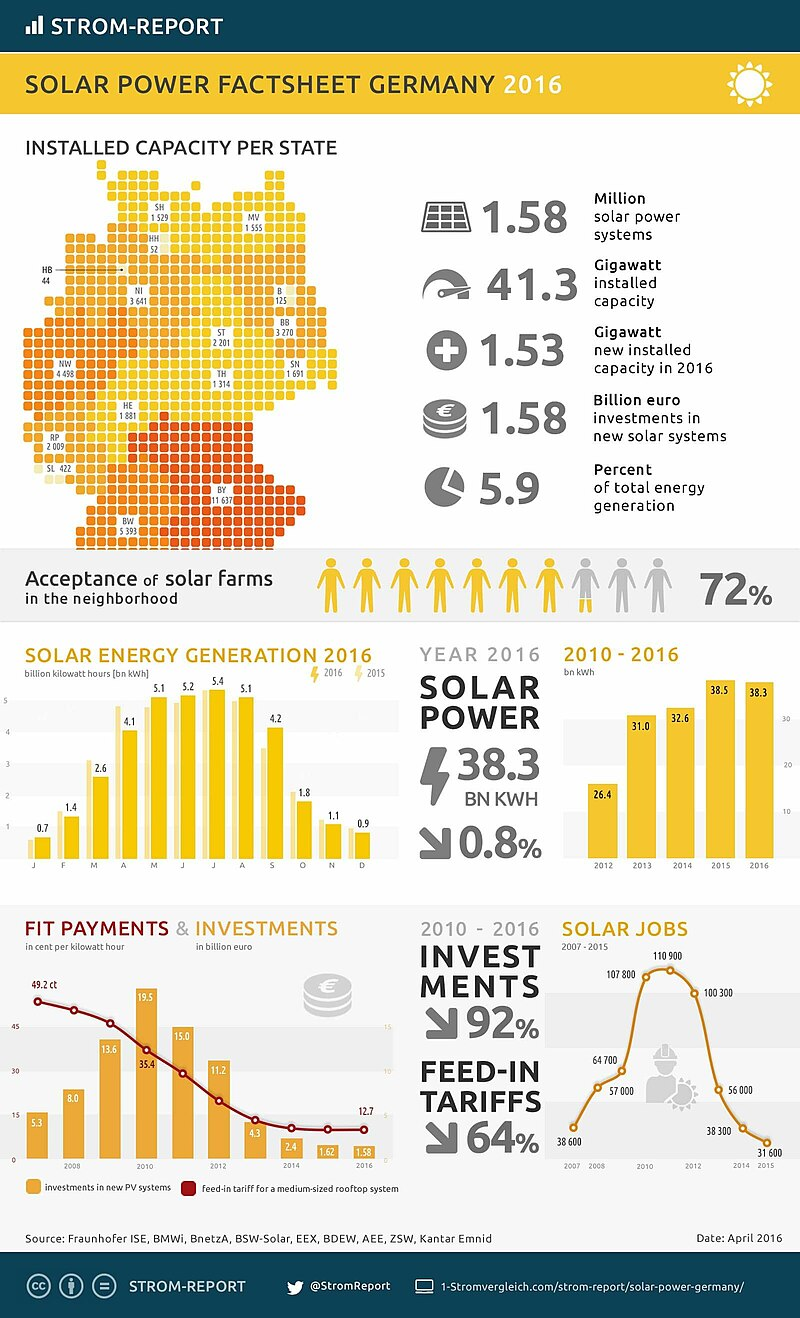
\includegraphics[width=4.5cm]{figures/solar_power.jpg}
\caption*{Credits: Strom Report}
\end{figure}
\end{minipage}
}
%
\frame{
\frametitle{Photons vs particles}
\begin{minipage}{0.5\linewidth}
\begin{itemize}
\item It will be essential to understand photon-matter interaction. As Ivan Hubeny said: 
\item \emph{...In other words radiation in fact determines the structure of the medium yet the medium is probed only by this radiation.}
\item Radiation: constituent in energy transport (and equation of state).
\item Also: diagnostics that allows us to understand physical properties of the medium.
\item Contrary to the lab: we need to treat wavelength and angular dependence of the radiation field.
\end{itemize}
\end{minipage}
\begin{minipage}{0.49\linewidth}
\begin{figure}
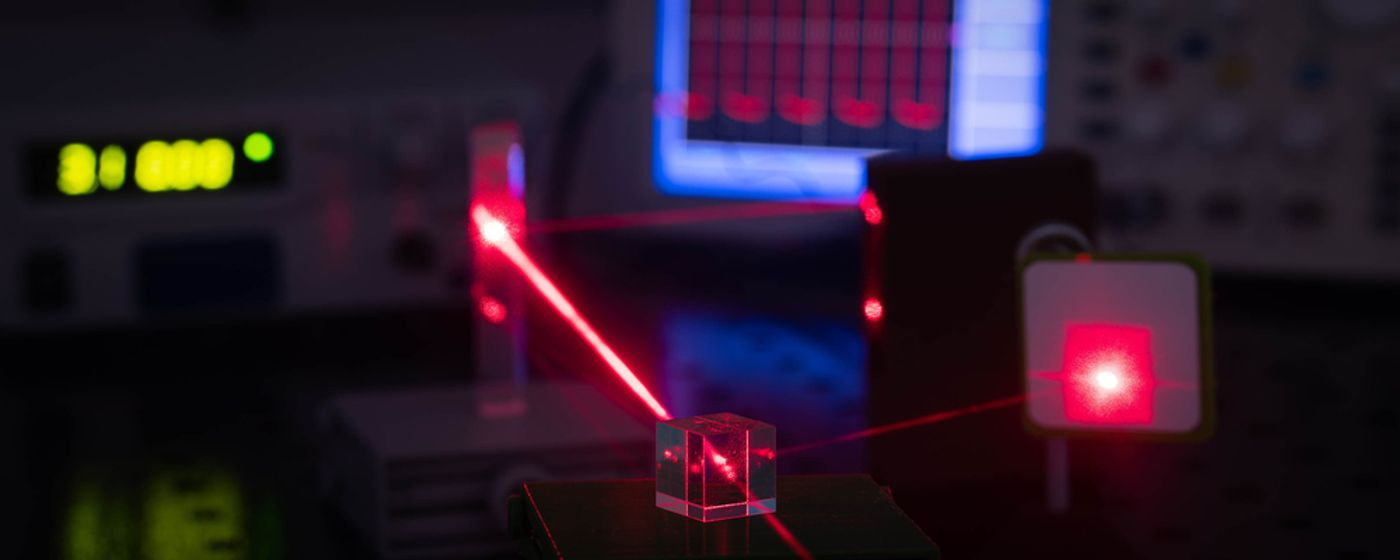
\includegraphics[width=4.5cm]{figures/laser_roots.jpg}\\
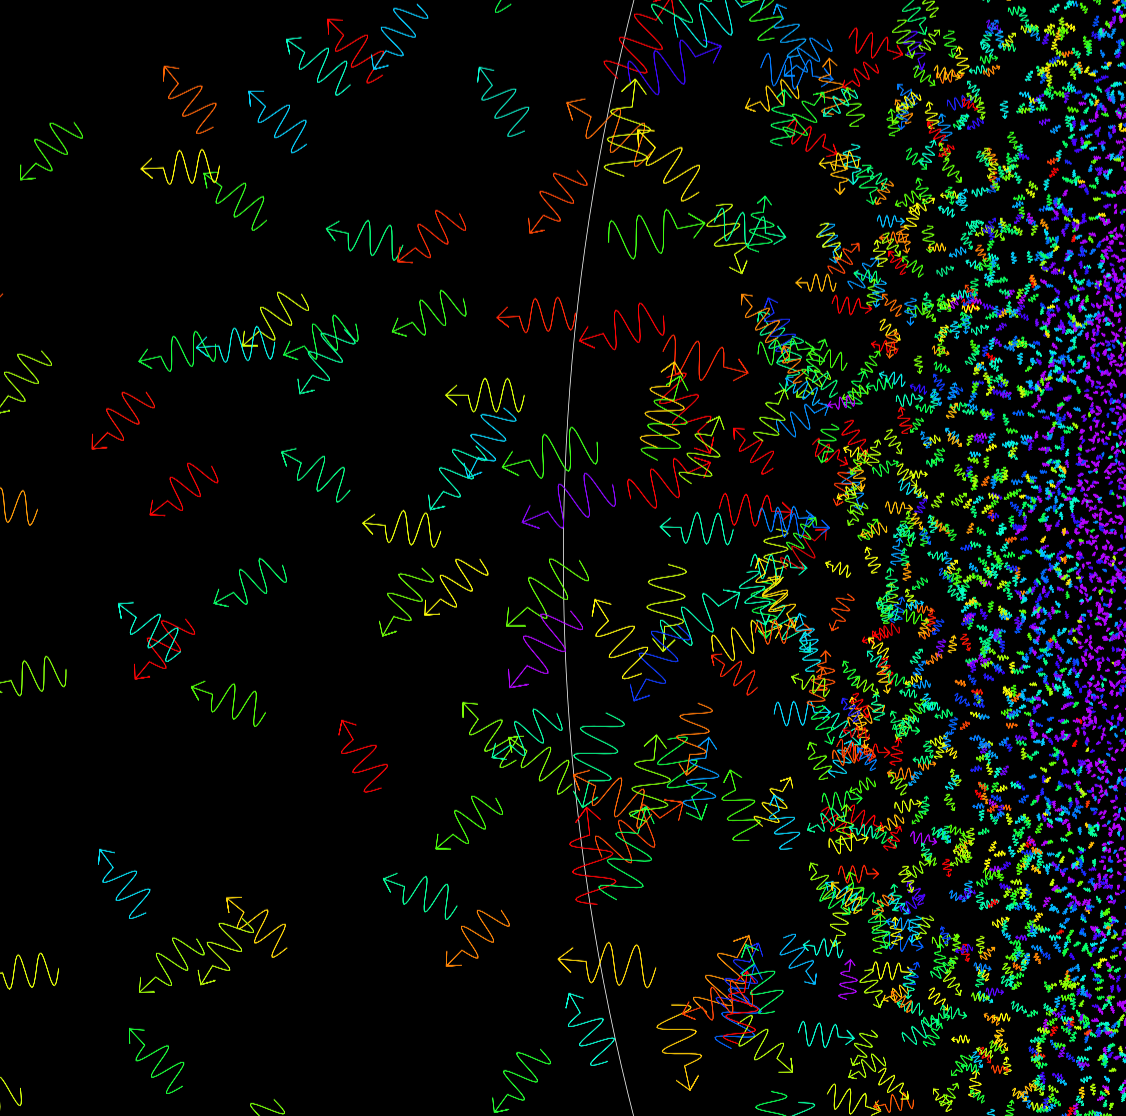
\includegraphics[width=4.5cm]{figures/sa.png}
\caption*{Credits: LabRoots.com (up), Prof. Rob Rutten (bottom)}
\end{figure}
\end{minipage}
}
%
\section{Radiation field}
%
\frame{
\frametitle{Specific monochromatic intensity}
\begin{minipage}{0.5\linewidth}
\begin{itemize}
\item We need to treat wavelength and angular dependence of the radiation field
\item Intensity: energy transported through given area in given time per given solid angle and frequency/wavelength bin (note the deprojection factor $\cos \theta$).
\begin{equation}
I_\nu = \frac{dE}{dS\,dt\,d\Omega\,d\nu\,\cos \theta}
\end{equation}
\item Going to number of photons:
\begin{equation}
n(\theta,\phi\,\nu) = \frac{I_\nu}{h\nu}
\end{equation}
\end{itemize}
\end{minipage}
\begin{minipage}{0.49\linewidth}
\begin{figure}
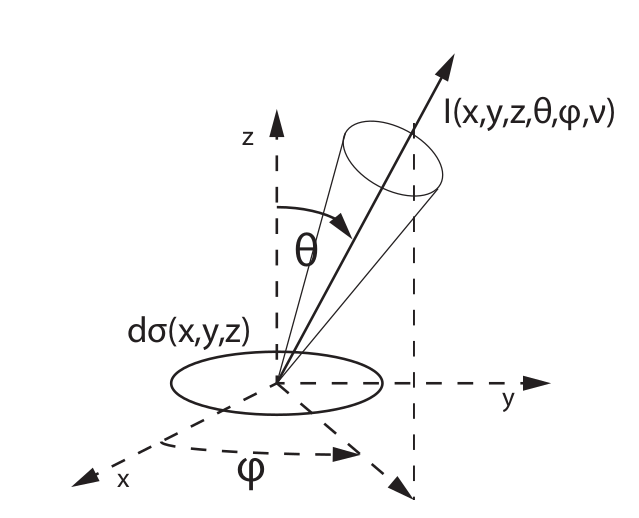
\includegraphics[width=6.0cm]{figures/spec_int.png}
\caption*{Credits: IM thesis (2014, University of Belgrade)}
\end{figure}
\end{minipage}
}
%
\frame{
\frametitle{Other ``moments'' of the radiation field}
\begin{minipage}{0.5\linewidth}
\begin{itemize}
\item Intensity fully describes the radiation field (without polarization). But often we need some derived quantities:
\item Mean intensity:
\begin{equation}
J_\nu = \frac{1}{4\pi}\oint I_\nu (\theta,\phi) \sin \theta d \theta d \phi
\end{equation}
\item Flux (in $z$ direction):
\begin{equation}
\mathcal{F}_\nu = \oint I_\nu (\theta,\phi) \cos \theta \sin \theta  d \theta d \phi
\end{equation}
\end{itemize}
\end{minipage}
\begin{minipage}{0.49\linewidth}
\begin{figure}
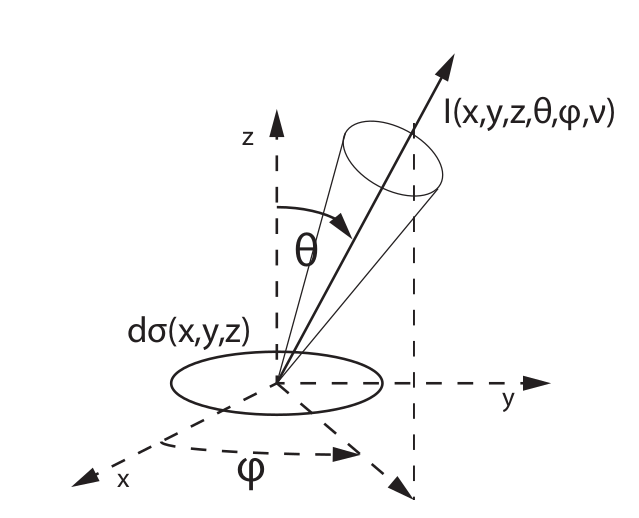
\includegraphics[width=6.0cm]{figures/spec_int.png}
\caption*{Credits: IM thesis (2014, University of Belgrade)}
\end{figure}
\end{minipage}
}
%
\frame{
\frametitle{Some de-confusion of the term flux}
\begin{itemize}
\item Typically we say that (spectral, monochromatic) flux is:
\begin{equation}
F_\nu = \frac{dE}{dt dS d\nu}
\end{equation}
\item But in the book typically:
\begin{equation}
F_\nu = \frac{dE}{dt d\nu} \rightarrow F = \frac{dE}{dt}
\end{equation}
But then, to make situation worse, in stellar atmospheres theory flux is:
\begin{equation}
\mathcal{F}_\nu = \frac{dE}{dt dS d\nu}
\end{equation}
then astrophysical flux: 
\begin{equation}
F_\nu = \frac{1}{\pi}\frac{dE}{dt dS d\nu}
\end{equation}
and Eddington flux (which the book uses and calls the radiation flux) is:
\begin{equation}
H_\nu = \frac{1}{4\pi}\frac{dE}{dt dS d\nu} = \frac{1}{4\pi} \mathcal{F}_\nu
\end{equation}
\end{itemize}
}
%
\frame{
\frametitle{More moments of the radiation field}
\begin{itemize}
\item Mean intensity:
\begin{equation}
J_\nu = \frac{1}{4\pi}\oint I_\nu (\theta,\phi) \sin \theta d \theta d \phi
\end{equation}
\item Radiation flux:
\begin{equation}
\mathcal{H}_\nu = \frac{1}{4\pi} \oint I_\nu (\theta,\phi) \cos \theta \sin \theta  d \theta d \phi
\end{equation}
\item and the so called K-integral, which is proportional to the pressure of the radiation field:
\begin{equation}
\mathcal{K}_\nu = \frac{1}{4\pi} \oint I_\nu (\theta,\phi) \cos^2 \theta \sin \theta  d \theta d \phi = \frac{p_\nu c}{4 \pi}
\end{equation}
\item \textbf{Note that we can define all these in the frequency/wavelength-integrated form}

\end{itemize}
}
%
%
\frame{
\frametitle{More moments of the radiation field}
\begin{itemize}
\item Mean intensity:
\begin{equation}
J = \frac{1}{4\pi}\int_0^{\infty}\oint I_\nu (\theta,\phi) \sin \theta d \theta d \phi d\nu
\end{equation}
\item Radiation flux:
\begin{equation}
\mathcal{H} = \frac{1}{4\pi} \int_0^{\infty}\oint I_\nu (\theta,\phi) \cos \theta \sin \theta  d \theta d \phi d\nu
\end{equation}
\item and the so called K-integral, which is proportional to the pressure of the radiation field:
\begin{equation}
\mathcal{K} = \frac{1}{4\pi} \int_0^{\infty}\oint I_\nu (\theta,\phi) \cos^2 \theta \sin \theta  d \theta d \phi d\nu = \frac{p\,c}{4 \pi} 
\end{equation}
\item \textbf{Here we integrated over all frequencies}

\end{itemize}
}
%
\frame{
\frametitle{A quick question:}
\begin{itemize}
\item What would be the radiation flux if the intensity was isotropic?
\begin{equation}
\mathcal{H}_\nu = \frac{1}{4\pi} \oint I_\nu (\theta,\phi) \cos \theta \sin \theta  d \theta d \phi
\end{equation}

\end{itemize}
}
%
%
\frame{
\frametitle{A quick question:}
\begin{itemize}
\item What would be the radiation flux if the intensity was isotropic?
\begin{equation}
\mathcal{H}_\nu = \frac{1}{4\pi} \oint I_\nu (\theta,\phi) \cos \theta \sin \theta  d \theta d \phi
\end{equation}
\item A common substitute in this case is to integrate $\phi$ to $2\pi$ and then set $\cos \theta = \mu$ (this is again an another $\mu$).
\begin{equation}
\mathcal{H}_\nu = \frac{1}{2} \int_{-1}^{1} I_\nu (\mu) \mu d\mu = 0
\end{equation}
\item If the radiation is completely isotropic, there is no energy transport. In order to transport the energy outward toward the surface the radiation has to be slightly anisotropic.
\end{itemize}
}
%
\section{RTE}
%
\frame{
\frametitle{Modeling the radiation field}
\begin{minipage}{0.5\linewidth}
\begin{itemize}
\item Our task is not to model and understand intensity and its relationship with other physical quantities (density, temperature, pressure, chemical composition). For that we need to:
\item Understand the interaction between the radiation and matter (absorption, emission, scattering coefficients).
\item Mathematically express relationship between these coefficients and the intensity. 
\end{itemize}
\end{minipage}
\begin{minipage}{0.49\linewidth}
\begin{figure}
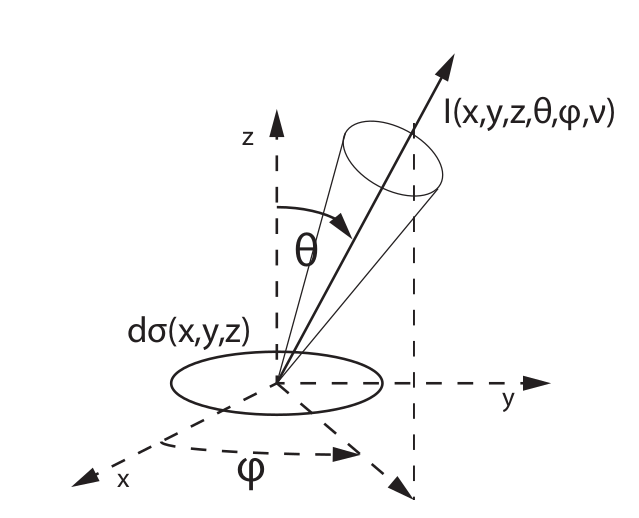
\includegraphics[width=6.0cm]{figures/spec_int.png}
\caption*{Credits: IM thesis (2014, University of Belgrade)}
\end{figure}
\end{minipage}
}
%
%
\frame{
\frametitle{Radiative Transfer Equation (RTE)}
\begin{minipage}{0.5\linewidth}
\begin{itemize}
\item This formulation is (more or less) due to Kirchhoff. The change of intensity ``along-the-ray'' over a distance $ds$ is:
\begin{equation}
dI_\nu = \eta_\nu ds - \chi_\nu I_\nu ds 
\end{equation} 
\item The terms of the right represent emission and \textbf{total} absorption (both true absorption and scattering) per unit volume.
\end{itemize}
\end{minipage}
\begin{minipage}{0.49\linewidth}
\begin{figure}
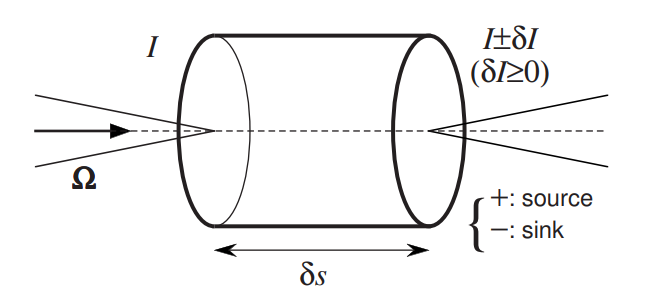
\includegraphics[width=6cm]{figures/rte_1.png}
\caption*{Credit: Anthony B. Davis and Yuri Knyazikhin}
\end{figure}
\end{minipage}
}
%
\frame{
\frametitle{Radiative Transfer Equation}
\begin{minipage}{0.55\linewidth}
\begin{itemize}
\item Now, it makes sense that the absorption and emission properties of the medium depend on:
\item Amount of matter capable of absorbing/emitting
\item The inherent properties of the matter at the given temperature ($T$ is very important!)
\item So we define:
\begin{align}
\kappa_\nu = \chi_\nu / \rho \\
j_\nu = \eta_\nu / \rho
\end{align}
\item So our equation becomes:
\begin{equation}
\frac{1}{\rho} \frac{dI_\nu}{ds} = -\kappa_\nu I_\nu + j_\nu
\end{equation}
\end{itemize}
\end{minipage}
\begin{minipage}{0.44\linewidth}
\begin{figure}
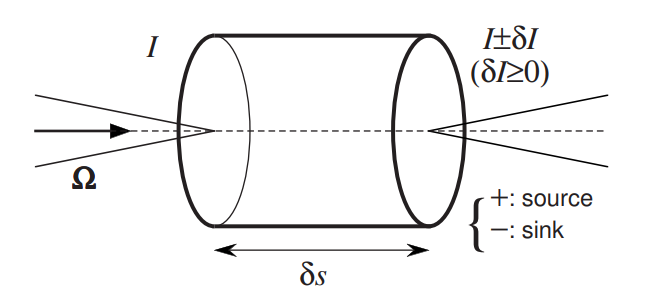
\includegraphics[width=6cm]{figures/rte_1.png}
\caption*{Credit: Anthony B. Davis and Yuri Knyazikhin}
\end{figure}
\end{minipage}
}
%
\frame{
\frametitle{Few remarks}
\begin{minipage}{0.55\linewidth}
\begin{itemize}
\item This equation does not involve any new physical laws, it is a mathematical tool.
\begin{equation}
\frac{1}{\rho} \frac{dI_\nu}{ds} = -\kappa_\nu I_\nu + j_\nu
\end{equation}
\item $ds$ is a so-called ``ray'', its relationship to $dx, dy, dz$ will depend on the geometry we choose and the context.
\item We will assume that coefficients of absorption and emission are isotropic, but that they do depend on the frequency / wavelength.
\item \textbf{The intensity is not isotropic. Can you see why?}.
\end{itemize}
\end{minipage}
\begin{minipage}{0.44\linewidth}
\begin{figure}
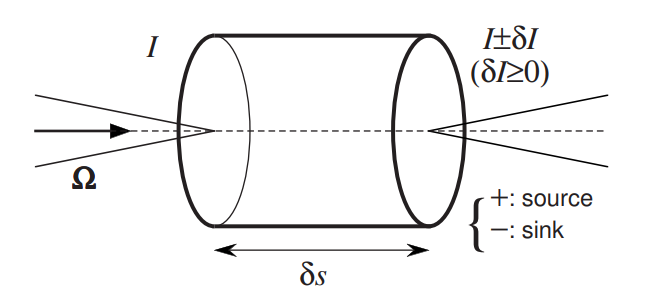
\includegraphics[width=6cm]{figures/rte_1.png}
\caption*{Credit: Anthony B. Davis and Yuri Knyazikhin}
\end{figure}
\end{minipage}
}
%
\frame{
\frametitle{RTE in 1D plane-parallel geometry}
\begin{minipage}{0.55\linewidth}
\begin{itemize}
\item If we assume that we are in 3D Cartesian grid, and nothing depends on $x$ and $y$, we will get:
\begin{equation}
ds = dz / \cos \theta = dr \cos \theta
\end{equation}
\item If we want to take the sphericity in context, this becomes more complicated, but we won't need it.
\item \textbf{In 1D, the anisotropy appears because $ds$ depends on the direction ($\theta$)}.
\end{itemize}
\end{minipage}
\begin{minipage}{0.44\linewidth}
\begin{figure}
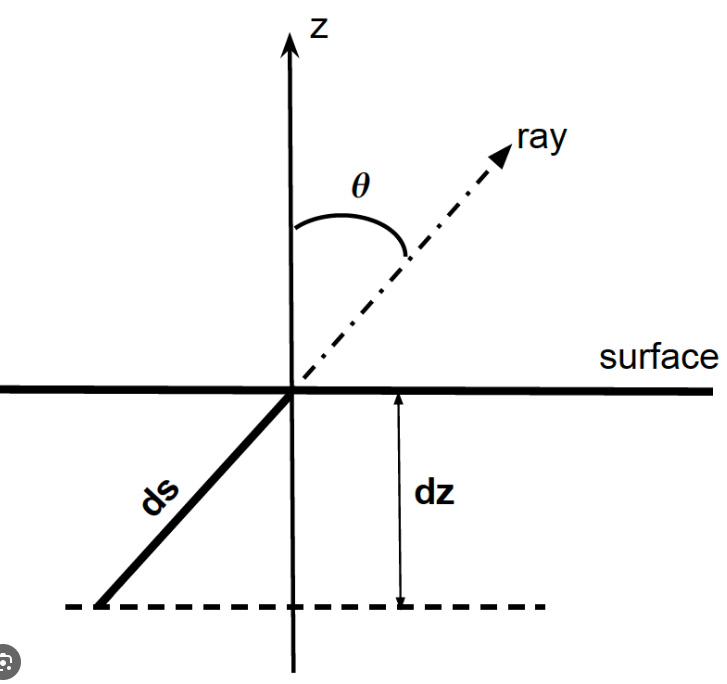
\includegraphics[width=6cm]{figures/ray.png}
\caption*{Credit: Frederic Paletou}
\end{figure}
\end{minipage}
}

\frame{
\frametitle{Optical depth and Source function}
\begin{minipage}{0.55\linewidth}
\begin{itemize}
\item We often do the following:
\begin{equation}
\frac{dI_\nu}{-\rho \kappa_\nu ds} = I_\nu - j_\nu / \kappa_\nu
\end{equation}
\item And we get:
\begin{equation}
\frac{dI_\nu}{-\rho \kappa_\nu ds} = I_\nu - j_\nu / (\rho \kappa_\nu)
\end{equation}

\begin{align}
\kappa_\nu = \chi_\nu / \rho; \,j_\nu = \eta_\nu / \rho
\end{align}
\item So our equation becomes:
\begin{equation}
\frac{dI_\nu}{d\tau_\nu} = I_\nu - S_\nu
\end{equation}
\end{itemize}
\end{minipage}
\begin{minipage}{0.44\linewidth}
\begin{figure}
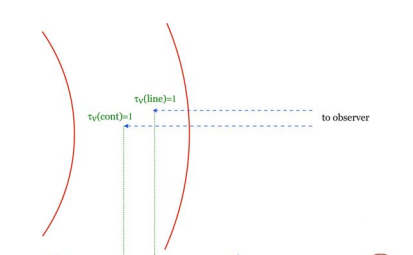
\includegraphics[width=6cm]{figures/tau.png}
\caption*{Credit: Rolf Kudritzki}
\end{figure}
\end{minipage}
}
%
\frame{
\frametitle{Optical depth and Source function}
\begin{minipage}{0.55\linewidth}
\begin{itemize}
\item If I wanted to be pedantic - I would have written:
\begin{equation}
\frac{dI_\nu(\theta)}{d\tau_\nu(\theta)} = I_\nu(\theta) - S_\nu
\end{equation}
\item A lot of interesting solutions will involve exponents of $\tau_\nu$ - nice that it is dimensionless.
\item For example, when there is no emission:
\begin{equation}
I_\nu(\tau_nu) = I_\nu^0 e^{-\tau_\nu}
\end{equation}
\item \q{Derive this real quick to get used to the orientation of optical depth.}
\end{itemize}
\end{minipage}
\begin{minipage}{0.44\linewidth}
\begin{figure}
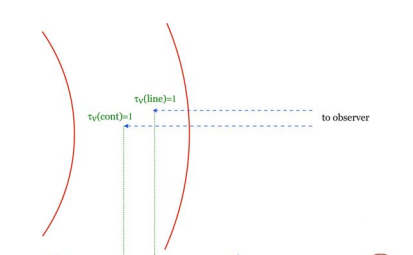
\includegraphics[width=6cm]{figures/tau.png}
\caption*{Credit: Rolf Kudritzki}
\end{figure}
\end{minipage}
}
%
\section{Kirchhoff Law and Planck Law}
\frame{
\frametitle{Kirchhoff Law}
\begin{minipage}{0.55\linewidth}
\begin{itemize}
\item Kirchhoff first wrote something like this and did a little thought experiment on a blackbody.
\begin{equation}
\frac{dI_\nu(\theta)}{d\tau_\nu(\theta)} = I_\nu(\theta) - S_\nu
\end{equation}
\item If the body is in a complete equilibrium, $dI_\nu$ is zero on every frequency, and $I_\nu$ is constant in space, and so is $T$. Then:
\begin{equation}
S_\nu = \frac{j_\nu}{\kappa_\nu} = f(T;\nu) = B_\nu(T)
\end{equation}
\item He argued that it is of utmost importance to find this function.
\end{itemize}
\end{minipage}
\begin{minipage}{0.44\linewidth}
\begin{figure}
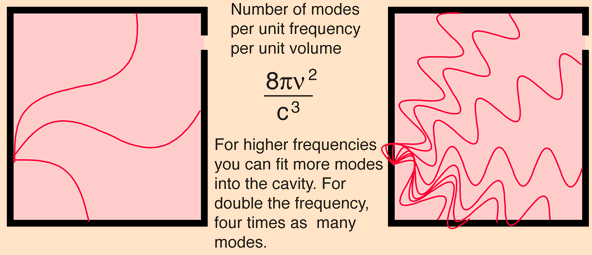
\includegraphics[width=6cm]{figures/cavity.png}
\caption*{Credit: Hyperphysics}
\end{figure}
\end{minipage}
}
% 
\frame{
\frametitle{Planck's Law}
\begin{minipage}{0.55\linewidth}
\begin{itemize}
\item People measured this function and Planck finally derived it (a nicer derivation is due to Bose and Einstein):
\begin{equation}
B_\nu(T) = \frac{2h\nu^3}{c^2} (e^{h\nu/kT} - 1)^{-1}
\end{equation}
\item This is, then, intensity of radiation inside of a blackbody. Integrating in wavelengths yields:
\begin{equation}
B(T) = {\rm const} T^4
\end{equation}
\item And finally integrating that in angle yields the good old $\sigma T^4$.
\end{itemize}
\end{minipage}
\begin{minipage}{0.44\linewidth}
\begin{figure}
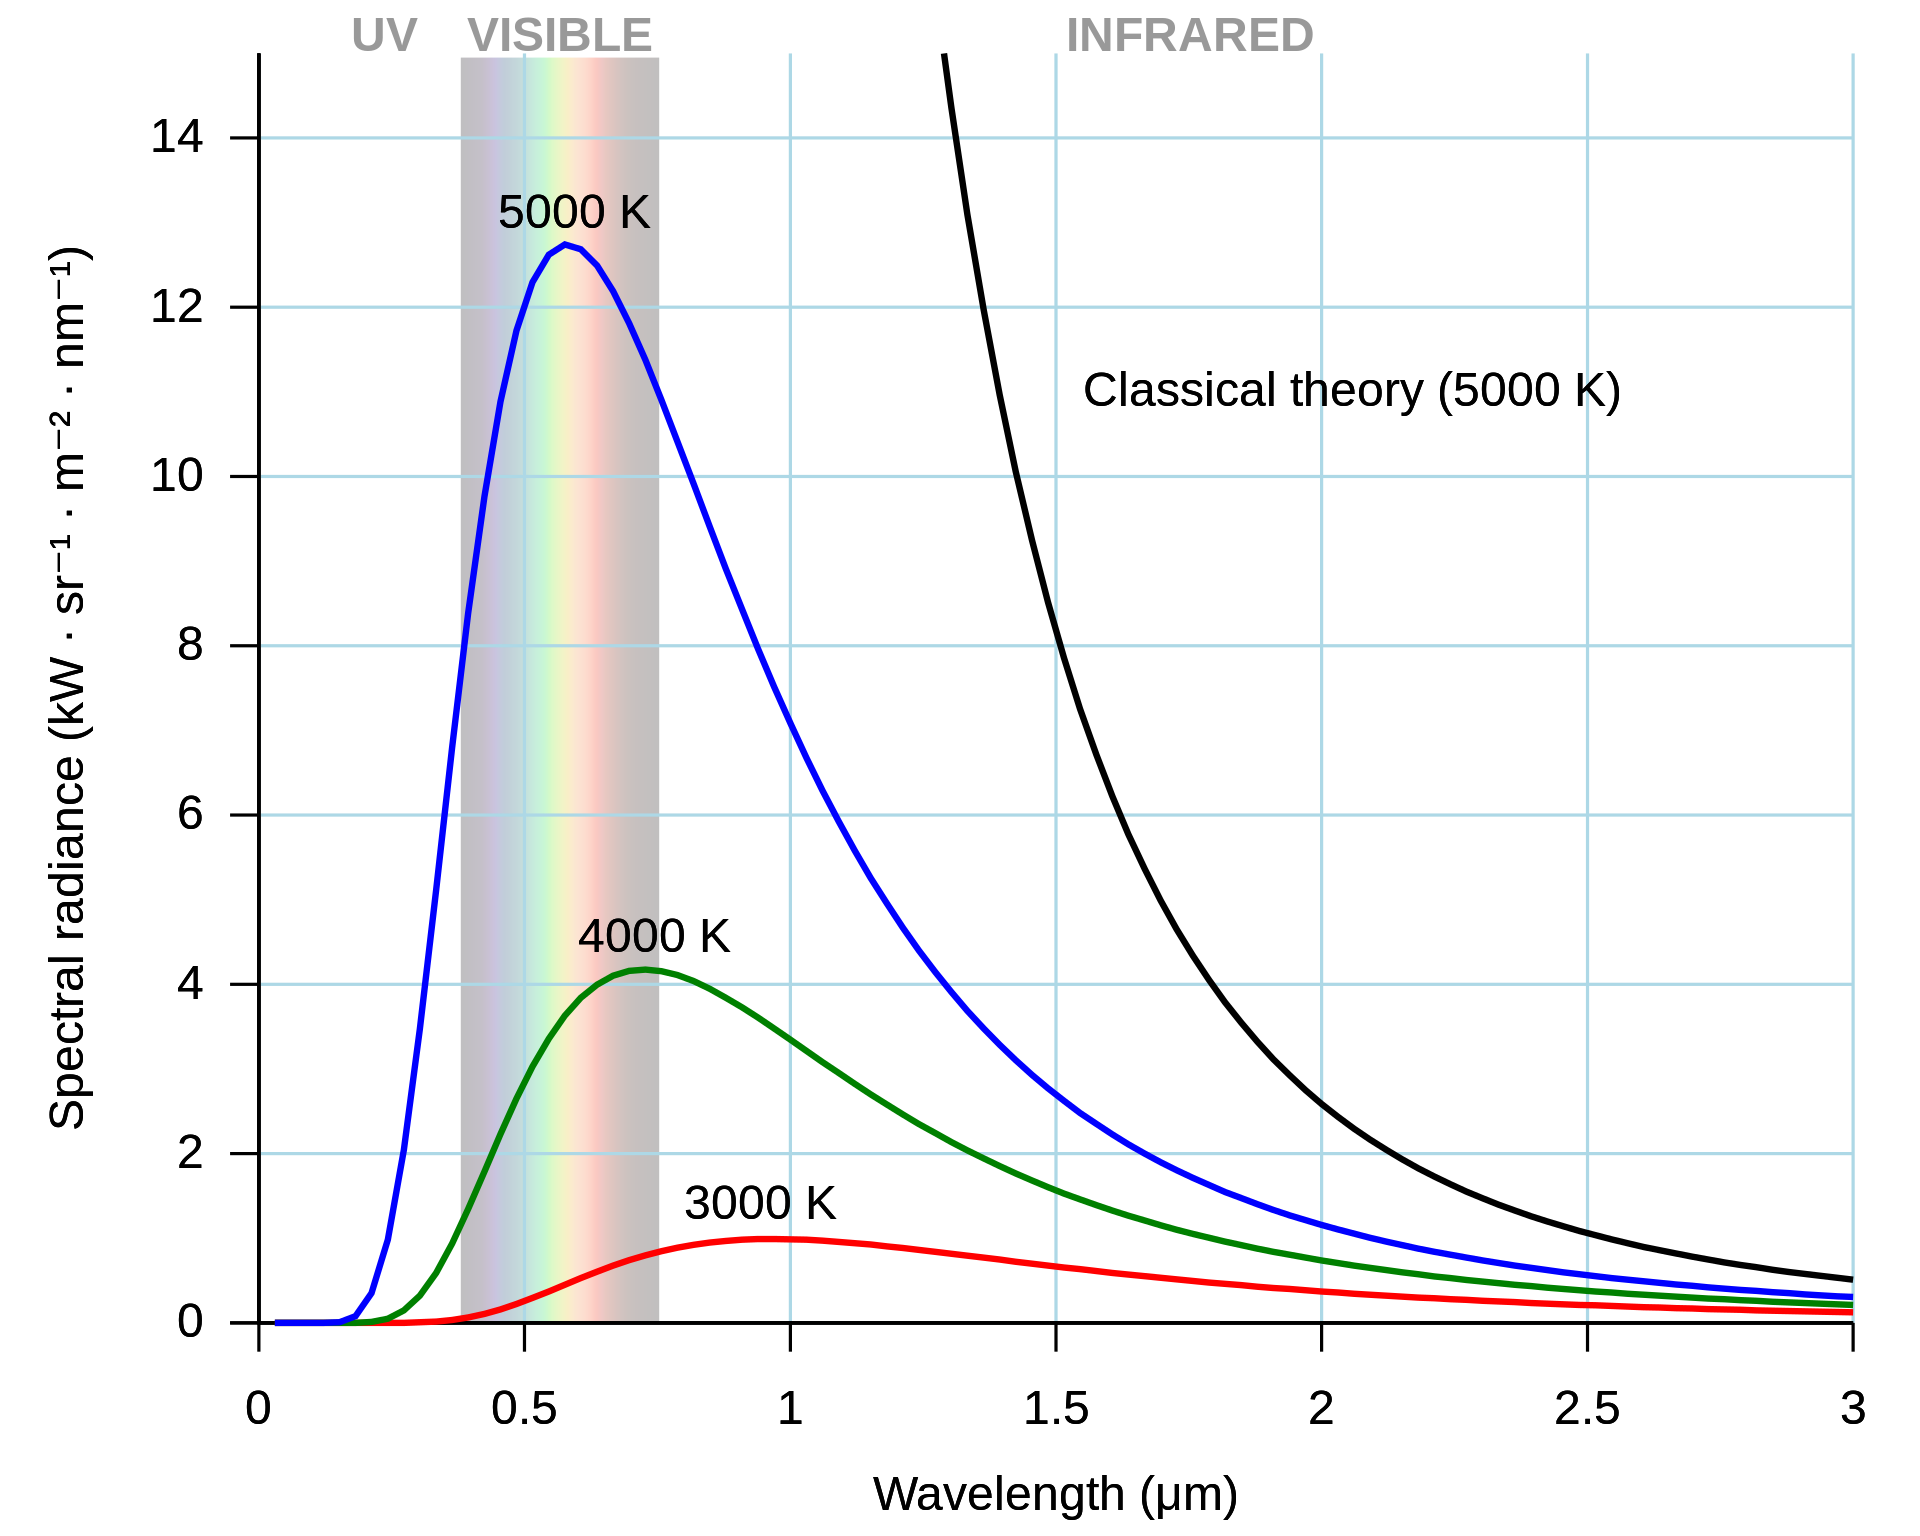
\includegraphics[width=6cm]{figures/bb.png}
\caption*{Credit: Wikipedia}
\end{figure}
\end{minipage}
}
% 
\frame{
\frametitle{But Ivan, stars are not black bodies}
\begin{minipage}{0.55\linewidth}
\begin{itemize}
\item If stars were blackbodies there would be no transport of energy.
\item However, the gradient of temperature in the stars is very small.
\item \q{Can you estimate?} (${\rm K/m}$?)
\end{itemize}
\end{minipage}
\begin{minipage}{0.44\linewidth}
\begin{figure}
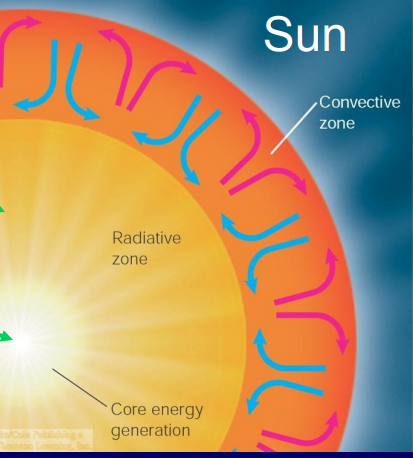
\includegraphics[width=6cm]{figures/star.png}
\caption*{Credits: George Blanford}
\end{figure}
\end{minipage}
}
% 
\frame{
\frametitle{Local Thermodynamic Equilibrium}
\begin{minipage}{0.55\linewidth}
\begin{itemize}
\item $dT/dr \approx 10^{-2} {\rm K/m}$ - This is incredibly small
\item This allows us to presume the so called \emph{local} thermodynamic equilibrium, which states that \textbf{matter} obeys:
\item Saha distribution over ionization states. 
\item Boltzmann distribution over excitation states. 
\item Maxwell distribution over velocities.
\item Contrary to what most of the textbooks tell you: \emph{radiation is not in equilibrium with matter} - Intensity has to be out of equilibrium or there is no energy transport.
\end{itemize}
\end{minipage}
\begin{minipage}{0.44\linewidth}
\begin{figure}
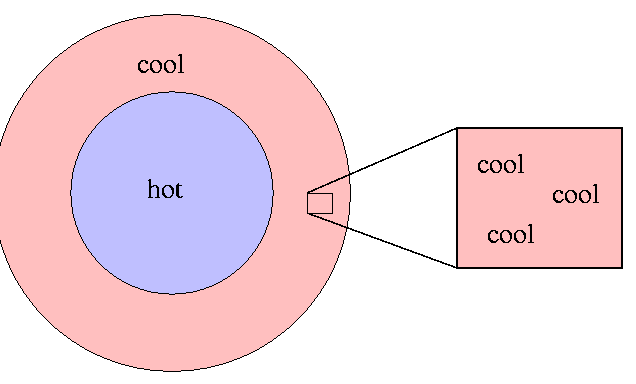
\includegraphics[width=6cm]{figures/lte.png}
\caption*{Credits: Michael Richmond}
\end{figure}
\end{minipage}
}
% 
% 
\frame{
\frametitle{Local Thermodynamic Equilibrium}
\begin{minipage}{0.55\linewidth}
\begin{itemize}
\item \emph{Radiation is not in equilibrium with matter} - Intensity has to be out of equilibrium or there is no energy transport.
\item But the source function, that depends only on the matter - is in equilibrium, and is equal to planck function:
\begin{equation}
S_\nu = B_\nu(T) = \frac{2h\nu^3}{c^2} (e^{h\nu/kT} - 1)^{-1}
\end{equation}
\item So, local emission and absorption properties of the material follow from equilibrium distributions but the radiation departs from it. 
\item This departure is very slight in the cores of the stars but can be huge in the outer layers. 
\item \q{Discuss the Sun's radiation that reaches us}.
\end{itemize}
\end{minipage}
\begin{minipage}{0.44\linewidth}
\begin{figure}
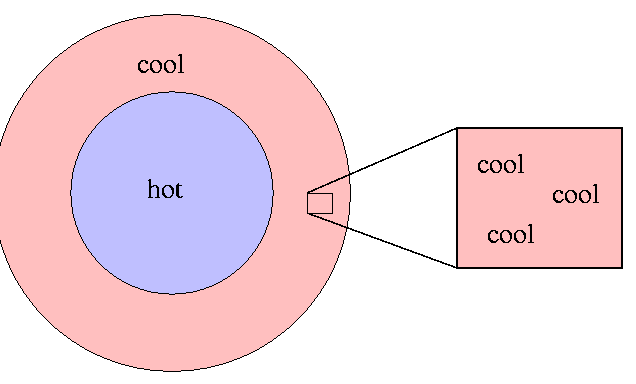
\includegraphics[width=6cm]{figures/lte.png}
\caption*{Credits: Michael Richmond}
\end{figure}
\end{minipage}
}
% 
\section{Solving RTE in stellar interiors}
\frame{
\frametitle{Solving RTE deep in the atmospheres}
\begin{minipage}{0.55\linewidth}
\begin{itemize}
\item We will not follow the approach from the book, but rather arguments used in stellar atmosphere modeling. (Still, very similar):
\begin{equation}
\cos \theta \frac{dI_\nu}{-\rho \kappa_\nu dz} = I_\nu - B_\nu
\end{equation}
\item Then we multiply the equation by $\cos \theta$ and integrate over all angles:
\begin{equation}
\frac{dK_\nu}{-\rho \kappa_\nu dz} = \mathcal{F}_\nu
\end{equation}
\item Here $K_\nu$ is the so called K-integral, which is proportional to the radiation pressure.
\end{itemize}
\end{minipage}
\begin{minipage}{0.44\linewidth}
\begin{figure}
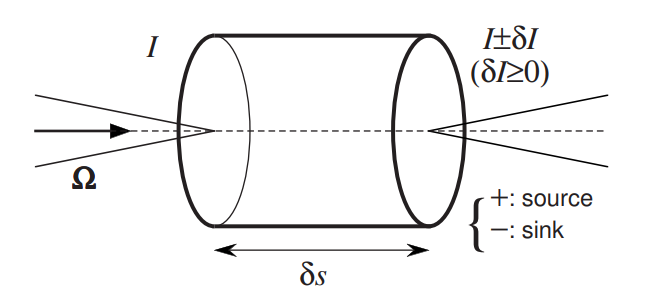
\includegraphics[width=6cm]{figures/rte_1.png}
\caption*{Credit: Anthony B. Davis and Yuri Knyazikhin}
\end{figure}
\end{minipage}
}
% 
\frame{
\frametitle{Solving RTE deep in the atmospheres}
\begin{minipage}{0.55\linewidth}
\begin{equation}
\frac{dp_\nu}{-\rho \kappa_\nu dz} = \mathcal{F}_\nu
\end{equation}
\begin{itemize}
\item Nice! Flux of the radiation is equal to the gradient in the radiation pressure.
\item Now, let's integrate this over the frequencies, and introduce mean opacity $\overline{\kappa}$:
\begin{equation}
H(z) = \frac{1}{4\pi} \mathcal{F}(z)= -\frac{4 a c T^3}{3 \overline{\kappa} \rho} \frac{dT}{dz}
\end{equation}
\end{itemize}
\end{minipage}
\begin{minipage}{0.44\linewidth}
\begin{figure}
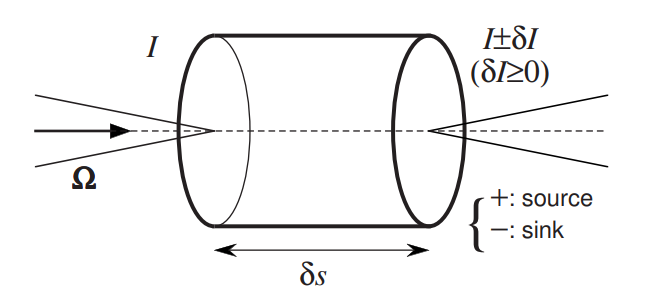
\includegraphics[width=6cm]{figures/rte_1.png}
\caption*{Credit: Anthony B. Davis and Yuri Knyazikhin}
\end{figure}
\end{minipage}
}
% 
\frame{
\frametitle{Radiative flux deep in the atmosphere:}
\begin{itemize}
\item If we now start from the book definition of $F$ ($F = 4\pi r^2 H$).
\begin{equation}
F = -4\pi r^2 \frac{4acT^3}{3\overline{\kappa} \rho} 
\end{equation}
\item Which we can invert to get:
\begin{equation}
\frac{dT}{dr} = - \frac{3}{4ac} \frac{\overline {\kappa}\rho}{T^3} \frac{F}{4\pi r^2}
\end{equation}
\item Or:
\begin{equation}
\frac{dT}{dm} = - \frac{3}{4ac} \frac{\overline {\kappa}}{T^3} \frac{F}{(4\pi r^2)^2}
\end{equation}
\item \q{Discuss and analyze!}
\item Obviously $\overline{\kappa}$ plays an important role here. Calculating it accurately as a function of $T$ and chemical compositon, for given $\rho$ is very very hard and important task!
\end{itemize}
}
% 
\frame{
\frametitle{What comes next?}
\begin{itemize}
\item Now, in principle we could move to upper layers and discuss radiative transfer in stellar atmospheres.
\item The situation there is trickier because things are much more anisotropic, and photons start escaping from the star. 
\item So, \textbf{frequency dependence is much more important}.
\item To prepare for that, and better understand the $\overline{\kappa}$, we will briefly discuss sources of absorption in the stars.
\end{itemize}
}
\section{Opacity sources}
% 
\frame{
\frametitle{What comes next?}
\begin{itemize}
\item In the execises we will see that: 
\begin{equation}
\frac{1}{\overline{\kappa}} = \frac{\int_0^{\infty} \frac{1}{\kappa_\nu} dB_\nu / dT d\nu}{\int_0^{\infty} dB_\nu / dT d\nu}
\end{equation} 

\item Therefore, we must understand the wavelength and temperature dependence of $\kappa_\nu$.
\item \q{Let's first talk about what contributes to $\kappa_\nu$}.
\end{itemize}
}
% 
\frame{
\frametitle{Opacity sources}
\begin{itemize}
\item Reminder, we only talk about opacity ($\kappa_\nu$) because $j_\nu = B_\nu \kappa_\nu$!
\item Some sources are:
\item Bound-free transitions (photoionization)
\item Free-free processes (inverse bremsstrahlung)
\item Bound-bound processes (spectral line - not important in the interior!)
\item Thomson and Rayleigh scattering. 
\item Photodissotiation of $H-$ and molecules.
\item Maybe some exotic processes?
\end{itemize}
}
% 
\frame{
\frametitle{Example: Bound-free processes}
\begin{minipage}{0.5\linewidth}
\begin{itemize}
\item To see the steps needed in the calculation of the opacity, try to solve the following problem
\item \q{For the gas of pure hydrogen, with given $\rho$ and $T$, calculate bound-free opacity at $\lambda$ = 50\,nm and 500\,nm}
\item First question: can hydrogen absorb these fotons?
\end{itemize}
\end{minipage}
\begin{minipage}{0.49\linewidth}
\end{minipage}
}
% 
\frame{
\frametitle{Example: Bound-free processes}
\begin{minipage}{0.5\linewidth}
\begin{itemize}
\item \q{For the gas of pure hydrogen, with given $\rho$ and $T$, calculate bound-free opacity at $\lambda$ = 50\,nm and 500\,nm}
\item For hydrogen to absorb, energy of the photon must be larger than the binding energy:
\begin{equation}
h\nu \ge E_i
\end{equation}
\end{itemize}
\end{minipage}
\begin{minipage}{0.49\linewidth}
\begin{figure}
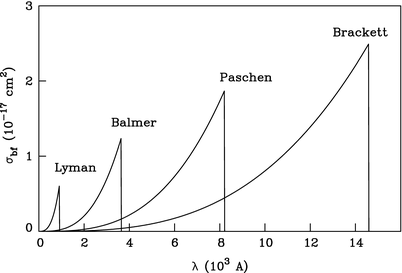
\includegraphics[width=6cm]{figures/hbf.png}
\caption*{Credit: Walter Maciel, Springer}
\end{figure}
\end{minipage}
}
%
\frame{
\frametitle{Example: Bound-free processes}
\begin{minipage}{0.5\linewidth}
\begin{itemize}
\item \q{For the gas of pure hydrogen, with given $\rho$ and $T$, calculate bound-free opacity at $\lambda$ = 50\,nm and 500\,nm}
\item For hydrogen to absorb, energy of the photon must be larger than the binding energy. 
\item But electrons at different bound states have different binding energies ($i$ is the excitation state)! 
\item Plus, not every wavelength is equally efficient!
\begin{equation}
h\nu \ge \frac{13.6 {\rm eV}}{i^2}
\end{equation}
\end{itemize}
\end{minipage}
\begin{minipage}{0.49\linewidth}
\begin{figure}
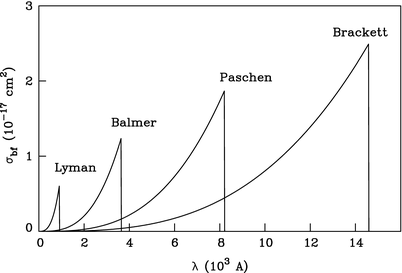
\includegraphics[width=6cm]{figures/hbf.png}
\caption*{Credit: Walter Maciel, Springer}
\end{figure}
\end{minipage}
}
%
\frame{
\frametitle{Example: Bound-free processes}
\begin{minipage}{0.5\linewidth}
\begin{itemize}
\item So, for given $\rho$ and $T$, we need to find number densities of all hydrogen atoms 
\item Ionized hydrogen does not contribute. 
\item Probably better if at this point we rely on the blackboard...
\item Plot on the right shows the \emph{cross-section} for various wavelengths.
\end{itemize}
\end{minipage}
\begin{minipage}{0.49\linewidth}
\begin{figure}
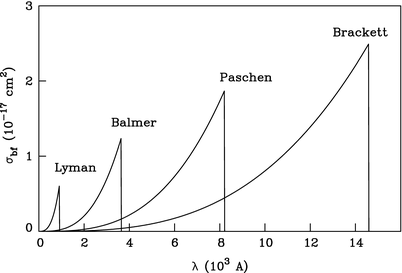
\includegraphics[width=6cm]{figures/hbf.png}
\caption*{Credit: Walter Maciel, Springer}
\end{figure}
\end{minipage}
}
%
\frame{
\frametitle{Result}
\begin{minipage}{0.5\linewidth}
\begin{itemize}
\item These calculations need to be done for a system of many elements.
\item Taking into account electron scattering.
\item Taking into account free-free processes (this is not scattering!)
\item Eventually, we will get the plot on the right
\item \q{What does the plot on the right tell us?}
\end{itemize}
\end{minipage}
\begin{minipage}{0.49\linewidth}
\begin{figure}
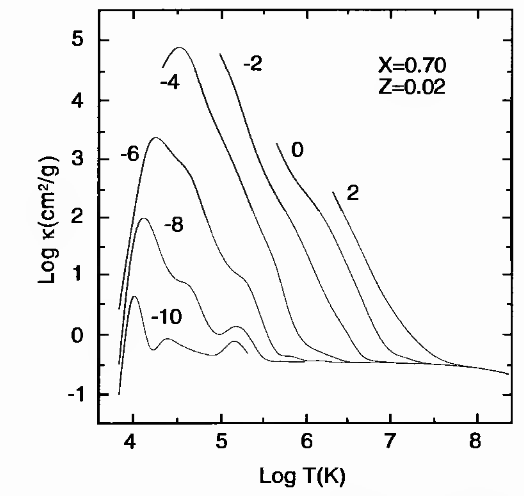
\includegraphics[width=6cm]{figures/op_table.png}
\caption*{Credit: Iglesias and Rogers (1996)}
\end{figure}
\end{minipage}
}
\end{document}
% 
\frame{
\frametitle{Summary}
\begin{itemize}
\item We have convinced ourselves that the radiation deep in the atmosphere diffuses and transports energy outward. 
\item Radiation and convection take place at different depths, depending on the physical conditions. 
\item Now, we are capable of talking about the solutions of the problem of stellar structure. 
\item We can also introduce time dependence to model stellar evolution.
\item Or we can complicate the radiative transfer, to understand stellar (and solar) atmospheres.
\item We will do a bit of everything in the upcoming lectures! 
\item \q{Discuss Friday}
\end{itemize}
}


